\documentclass[letterpaper,10pt]{article}
\usepackage[margin=2cm]{geometry}

\usepackage{graphicx}
\usepackage{amsmath}
\usepackage{amsfonts}
\usepackage{amssymb}
\usepackage[colorlinks]{hyperref}

\title{\textbf{18794 Pattern Recognition Theory\\Prof. Marios Savvides}}
\author{HMW-Alexander}

\begin{document}
	
\maketitle

\tableofcontents

\begin{center}\rule{\textwidth}{1pt}\end{center}
\section{Introduction}

\begin{center}\rule{\textwidth}{1pt}\end{center}
\section{Decision Theory}

\subsection{Terms}

\begin{itemize}
	\item Feature Space:
	\begin{itemize}
		\item \textbf{Feature}: a distinctive characteristic or quality of the object
		\item \textbf{Feature vector}: combine more than one feature as a vector
		\item \textbf{Feature space}: The space defined by the feature vectors
	\end{itemize}
	\item Classifiers:
	\begin{itemize}
		\item \textbf{Decision regions}: a classifier partitions the feature space into class-corresponding decision regions.
		\item \textbf{Decision boundaries}: the borders between the decision regions.
	\end{itemize}
\end{itemize}

\subsection{Bayes Rule}

\begin{equation}
P(w_i|x)=\frac{P(x,w_i)}{P(x)}=\frac{P(x|w_i)P(w_i)}{\sum_{k=1}^{C}{P(x|w_k)P(w_k)}}
\end{equation}
\begin{itemize}
	\item \textbf{Posterior Probability} $P(w_i|x)$: the conditional probability of correct class being $w_i$ given that feature value $x$ has been observed.
	\item \textbf{Evidence} $P(x)$: the total probability of observing the feature value of $x$.
	\item \textbf{Likelihood} $P(x|w_i)$: the conditional probability of observing a feature value of $x$ given that the correct class is $w_i$.
	\item \textbf{Prior Probability} $P(w_i)$: the probability of class $w_i$, $\sum_{k=1}^{C}{P(w_k)}=1$.
	\item \textbf{Bayes Classifiers} decide on the class that has the \textbf{largest posterior probability} ($\max_{w_i}{P(w_i|x)}$). They are statistically the best classifiers i.e. they are minimum error classifiers (optimal).
\end{itemize}

\subsection{Minimum Probability of Error}

\begin{itemize}
	\item $\epsilon=P(error|class)$: probability of assigning $x$ to the wrong class $w$.
	\item $P_e=\sum_{k=1}^{C}{P(w_k)\epsilon_k}$: total probability of error.
\end{itemize}
\begin{figure}[!ht]
	\centering
	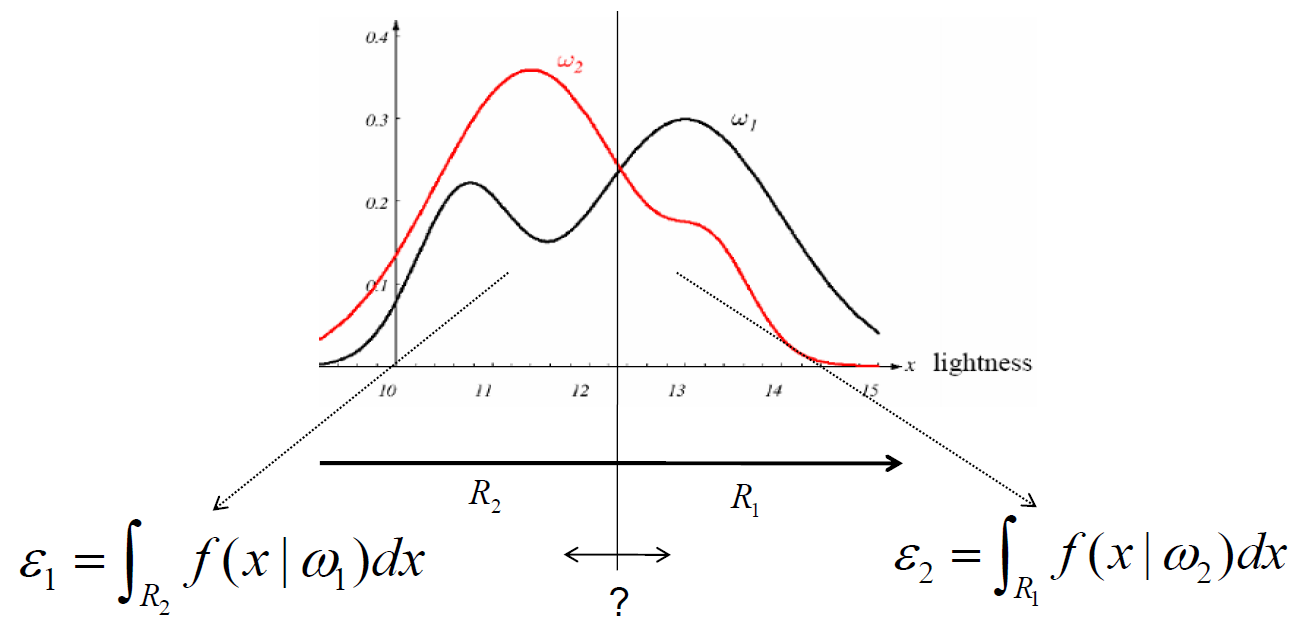
\includegraphics[width=10cm]{./img/minimum_probability_of_error.png}
\end{figure}
For the two class case shown above, we want to minimize $P_e$ as below:
\begin{equation}
\begin{array}{rcl}
P_e & = & P(w_1)\epsilon_1 + P(w_2)\epsilon_2 \\
	& = & P(w_1)\int_{R_2}{f(x|w_1)dx} + P(w_2)\int_{R_1}{f(x|w_2)dx} \\
	& = & P(w_1)(1-\int_{R_1}{f(x|w_1)dx}) + P(w_2)\int_{R_1}{f(x|w_2)dx} \\
	& = & P(w_1) + \int_{R_1}{(P(w_2)f(x|w_2) - P(w_1)f(x|w_1))dx} \\ 
\end{array}
\end{equation}
To minimize $P_e$, we want $P(w_2)f(x|w_2) - P(w_1)f(x|w_1)$ to be always negative$(<0)$ in the region $R_1$:
\begin{equation}
\begin{array}{rcl}
P(w_1)f(x|w_1) - P(w_2)f(x|w_2) >0 & \Rightarrow & w_1 \\
P(w_1)f(x|w_1) - P(w_2)f(x|w_2) <0 & \Rightarrow & w_2 \\
\end{array}
\end{equation}

\subsection{Likelihood Ratio}

\begin{itemize}
	\item \textbf{Likelihood ratio}: $l(x)=\frac{f(x|w_1)}{f(x|w_2)}$
	\item \textbf{Log likelihood ratio}: $ln(l(x))=ln(\frac{f(x|w_1)}{f(x|w_2)})=ln(f(x|w_1))-ln(f(x|w_2))$
	\item \textbf{Ratio of a priori probabilities}: $T=\frac{P(w_2)}{P(w_1)}$
	\item \textbf{Log ratio of a priori probabilities}: $ln(T)=ln(\frac{P(w_2)}{P(w_1)})=ln(P(w_2))-ln(P(w_1))$
\end{itemize}

\begin{equation}
\begin{array}{rcl}
ln(l(x)) = ln(\frac{f(x|w_1)}{f(x|w_2)}) > ln(\frac{P(w_2)}{P(w_1)}) = ln(T) & \Rightarrow & w_1 \\
ln(l(x)) = ln(\frac{f(x|w_1)}{f(x|w_2)}) < ln(\frac{P(w_2)}{P(w_1)}) = ln(T) & \Rightarrow & w_2 \\
\end{array}
\end{equation}

\subsubsection{Likelihood as Gaussian distribution}
Assume likelihood $f(x|w_i)$ are Gaussian distributions with mean $\mu_i$ and variance $\sigma_i^2$.
\begin{equation}
f(x|w_i)=\frac{1}{\sqrt{2\pi\sigma_i^2}}\exp\left(-\frac{(x-\mu_i)^2}{2\sigma_i^2}\right)
\end{equation}
\begin{figure}[!ht]
	\centering
	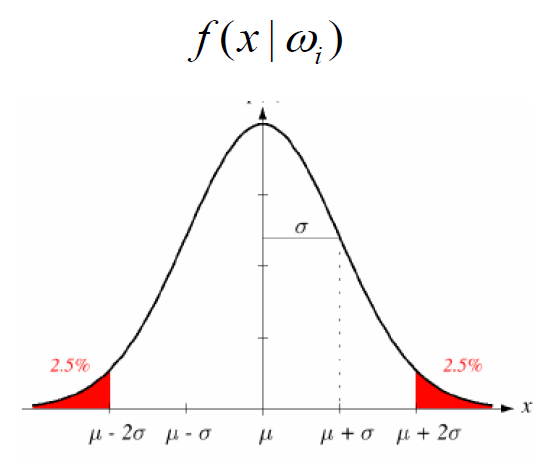
\includegraphics[width=6cm]{./img/gaussian_distribution_likelihood.png}
\end{figure}
The log likelihood ratio:
\begin{equation}
\begin{array}{rcl}
ln(l(x)) & = & ln\left(\frac{\frac{1}{\sqrt{2\pi\sigma_1^2}}\exp\left(-\frac{(x-\mu_1)^2}{2\sigma_1^2}\right)}{\frac{1}{\sqrt{2\pi\sigma_2^2}}\exp\left(-\frac{(x-\mu_2)^2}{2\sigma_2^2}\right)}\right) \\
         & = & ln(\frac{\sigma_2}{\sigma_1})+\frac{(x-\mu_2)^2}{2\sigma_2^2}-\frac{(x-\mu_1)^2}{2\sigma_1^2}
\end{array}
\end{equation}

Case: $\sigma_1=\sigma_2=\sigma$
\begin{equation}
\begin{array}{rcl}
ln(l(x)) & = & \frac{2x(\mu_1-\mu_2)-(\mu_1^2-\mu_2^2)}{2\sigma^2}
\end{array}
\end{equation}

\begin{equation}
\begin{array}{rcl}
x(\mu_1-\mu_2) - \frac{\mu_1^2-\mu_2^2}{2} > \sigma^2 ln(\frac{P(w_2)}{P(w_1)}) & \Rightarrow & w_1 \\
x(\mu_1-\mu_2) - \frac{\mu_1^2-\mu_2^2}{2} < \sigma^2 ln(\frac{P(w_2)}{P(w_1)}) & \Rightarrow & w_2 \\
\end{array}
\end{equation}

If $P(w_1)=P(w_2)$
\begin{equation}
x = \frac{\mu_1+\mu_2}{2}
\end{equation}

\begin{figure}[!ht]
	\centering
	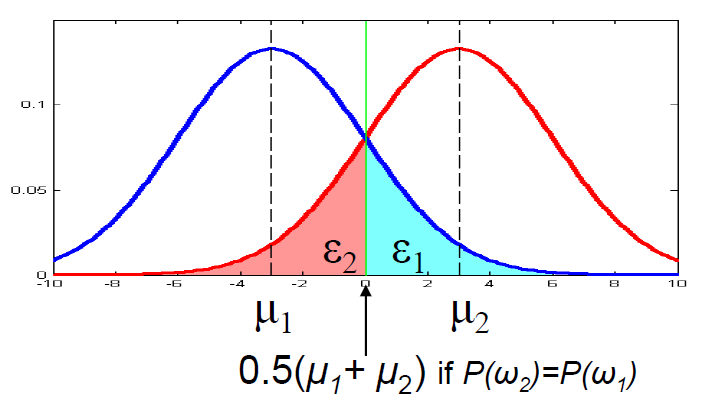
\includegraphics[width=8cm]{./img/gaussian_linear_classifier.png}
\end{figure}

Case: $\sigma_1\neq\sigma_2$

\begin{figure}[!ht]
	\centering
	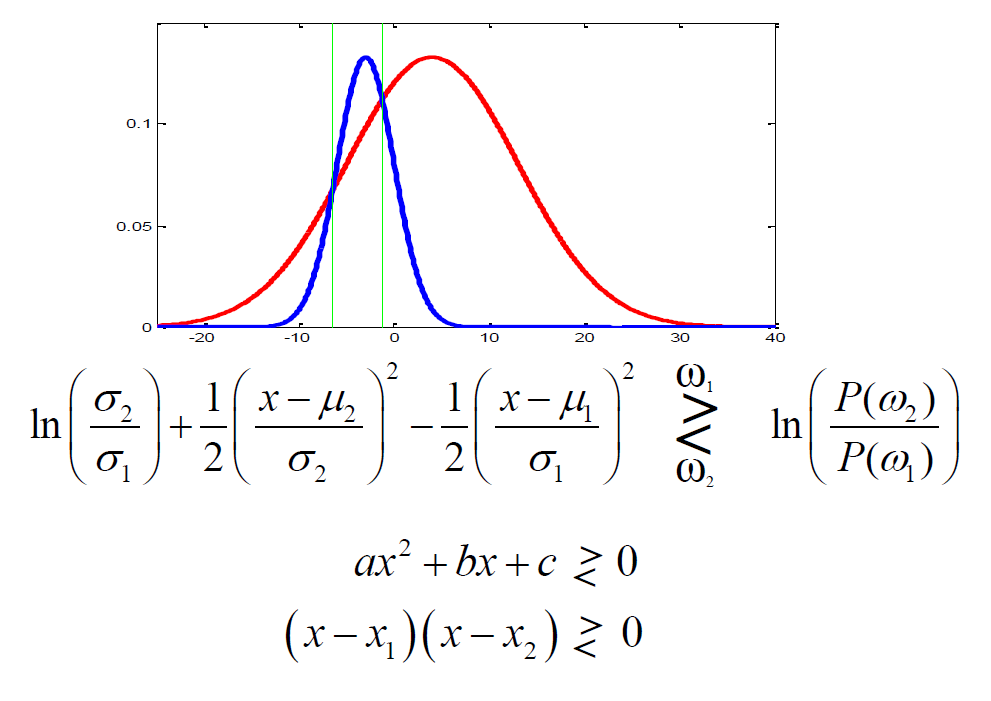
\includegraphics[width=8cm]{./img/guassian_quadratic_classifier.png}
\end{figure}

\end{document}